\documentclass{article}
\usepackage{amsmath,amssymb}
\usepackage{graphicx}
\usepackage{enumerate}
\usepackage{hyperref}
\usepackage{subcaption}
\usepackage{caption}
\usepackage{xcolor}
\usepackage{float}

\pagestyle{empty} \addtolength{\textwidth}{1.0in}
\addtolength{\textheight}{0.5in}
\addtolength{\oddsidemargin}{-0.5in}
\addtolength{\evensidemargin}{-0.5in}
\newcommand{\ruleskip}{\bigskip\hrule\bigskip}
\newcommand{\nodify}[1]{{\sc #1}}
\newcommand{\points}[1]{{\textbf{[#1 points]}}}
\newcommand{\subquestionpoints}[1]{{[#1 points]}}
\newenvironment{answer}{{\bf Answer:} \sf }{}%

\newcommand{\bitem}{\begin{list}{$\bullet$}%
{\setlength{\itemsep}{0pt}\setlength{\topsep}{0pt}%
\setlength{\rightmargin}{0pt}}}
\newcommand{\eitem}{\end{list}}

\setlength{\parindent}{0pt} \setlength{\parskip}{0.5ex}
\setlength{\unitlength}{1cm}

\newcommand{\pa}[1]{[[PA: #1]]}

\renewcommand{\Re}{{\mathbb R}}
\newcommand{\E}{{\rm E}}
\begin{document}

\pagestyle{myheadings} \markboth{}{CS 294-158 Deep Unsupervised Learning, Homework 4, Spring 2024}

{\huge
\noindent Homework 4: Diffusion Models}
\ruleskip

{\bf Deliverable}: This PDF write-up by {\bf Wednesday March 20th, 23:59pm}.  Your PDF should be generated by simply replacing the placeholder images of this LaTeX document with the appropriate solution images that will be generated automatically when solving each question. The solution images are automatically generated and saved using the accompanying IPython notebook. Your PDF is to be submitted into Gradescope. This PDF already contains a few solution images.  These images will allow you to check your own solution to ensure correctness.


\vspace{.2in}

%--------------------------------------------------------------------------------
%--------------------------------------------------------------------------------
%--------------------------------------------------------------------------------
\noindent {\bf Question 1: Toy Dataset [30pt]}
%--------------------------------------------------------------------------------
%--------------------------------------------------------------------------------
%--------------------------------------------------------------------------------

Final Test Loss: \textbf{0.3647} \\
\begin{figure}[H]
    \centering
    \begin{subfigure}{0.5\textwidth}
        \centering
        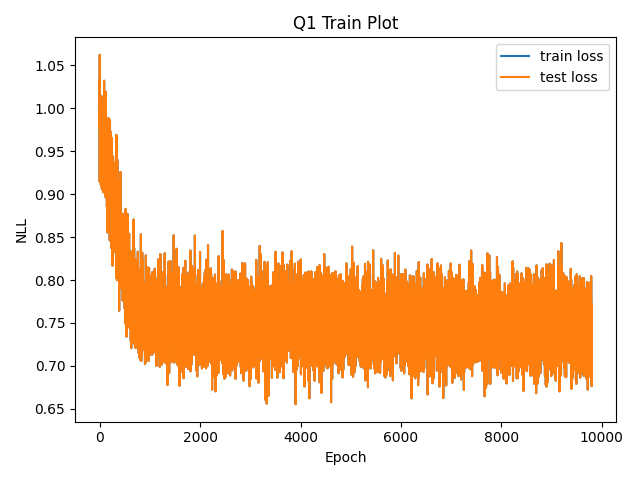
\includegraphics[width=\textwidth]{figures/q1_train_plot.png}
        \caption{Training curve}
    \end{subfigure}
    \\
    \begin{subfigure}{0.5\textwidth}
        \centering
        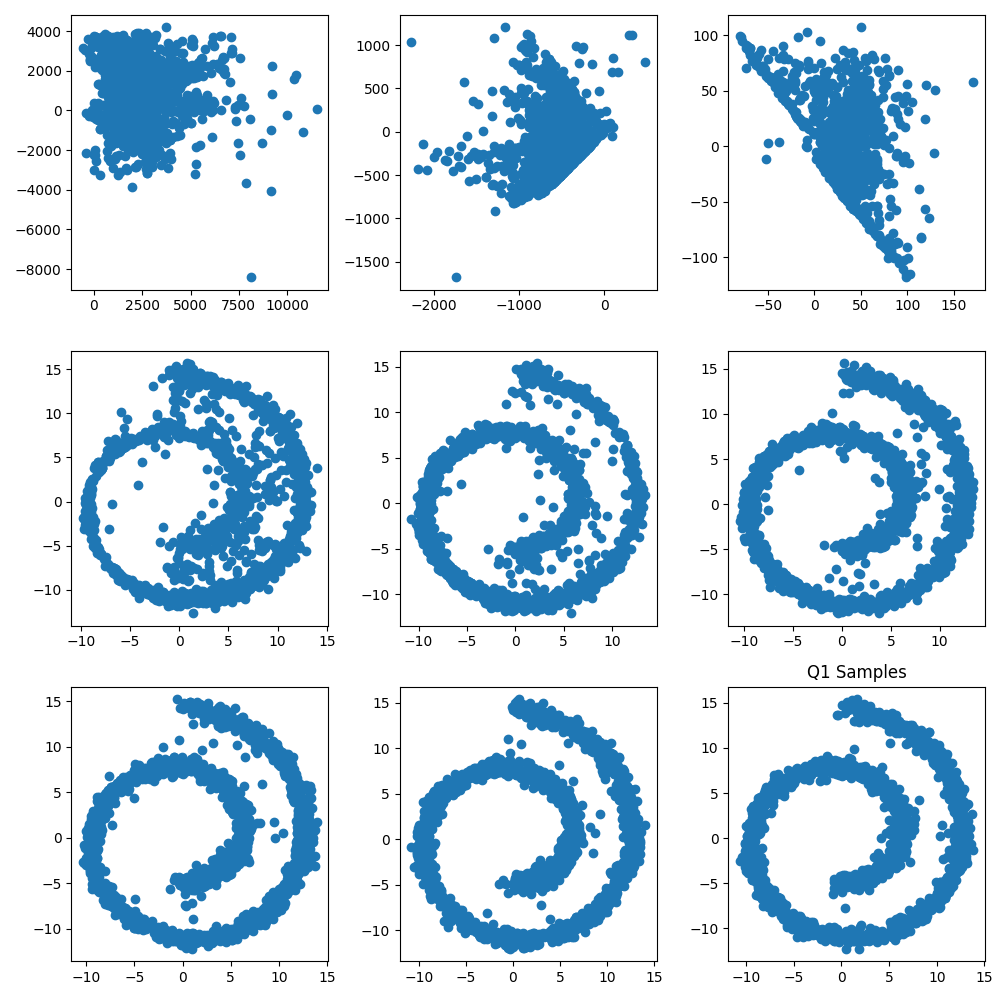
\includegraphics[width=\textwidth]{figures/q1_samples.png}
        \caption{Samples}
    \end{subfigure}
    
\end{figure}


%--------------------------------------------------------------------------------
%--------------------------------------------------------------------------------
%--------------------------------------------------------------------------------
\newpage
\noindent {\bf Question 2: Pixel-Space Diffusion on CIFAR-10 [30pt]} \\
%--------------------------------------------------------------------------------
%--------------------------------------------------------------------------------
%--------------------------------------------------------------------------------

    
Final Test Loss: \textbf{0.9999} \\
\begin{figure}[H]
    \centering
    \begin{subfigure}{0.7\textwidth}
        \centering
        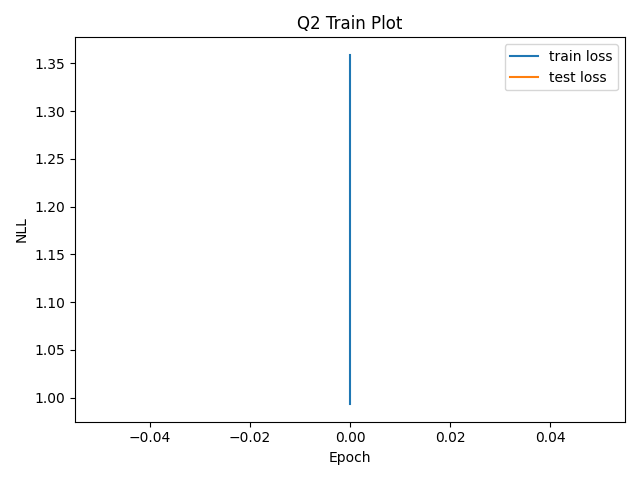
\includegraphics[width=\textwidth]{figures/q2_train_plot.png}
        \caption{Training curve}
    \end{subfigure}
    \\
    \begin{subfigure}{0.7\textwidth}
        \centering
        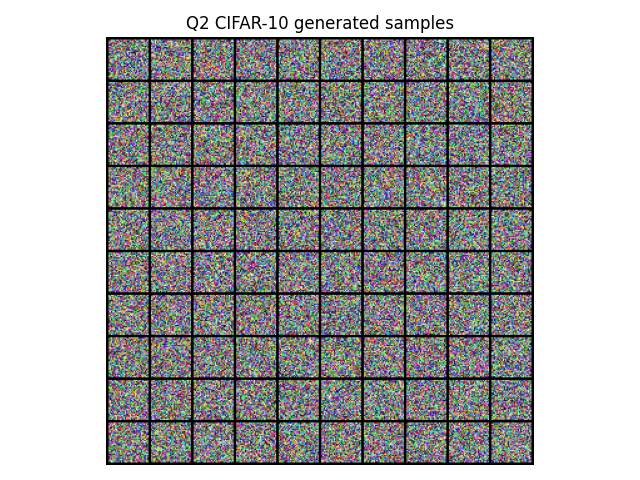
\includegraphics[width=\textwidth]{figures/q2_samples.png}
        \caption{Samples}
    \end{subfigure}
    
\end{figure}


%--------------------------------------------------------------------------------
%--------------------------------------------------------------------------------
%--------------------------------------------------------------------------------
\newpage
\noindent {\bf Question 3: Latent-Space Diffusion on CIFAR-10 with DiT [60 pt]}\\
%--------------------------------------------------------------------------------
%--------------------------------------------------------------------------------
%--------------------------------------------------------------------------------

\noindent {\bf Part a: VAE reconstructions and Scale Factor [10 pt]}\\
Scale factor: \textbf{TODO} \\
\begin{figure}[H]
    \centering
    \includegraphics[width=\textwidth]{figures/q3_a_reconstructions.png}
    \caption{Reconstructions}
\end{figure}

\newpage
\noindent {\bf Part b: Diffusion Transformer [30 pt]}\\
Final Test Loss: \textbf{TODO} \\
\begin{figure}[H]
    \centering
    \begin{subfigure}{0.7\textwidth}
        \centering
        \includegraphics[width=\textwidth]{figures/q3_b_train_plot.png}
        \caption{Training curve}
    \end{subfigure}
    \\
    \begin{subfigure}{0.7\textwidth}
        \centering
        \includegraphics[width=\textwidth]{figures/q3_b_samples.png}
        \caption{Samples}
    \end{subfigure}
\end{figure}

\newpage
\noindent {\bf Part c: Classifier-Free Guidance [20 pt]}
\begin{figure}[H]
    \centering
    \begin{subfigure}{0.45\textwidth}
        \centering
        \includegraphics[width=\textwidth]{figures/q3_c_samples_cfg1.0.png}
        \caption{Samples (CFG 1.0)}
    \end{subfigure}
    \begin{subfigure}{0.45\textwidth}
        \centering
        \includegraphics[width=\textwidth]{figures/q3_c_samples_cfg3.0.png}
        \caption{Samples (CFG 3.0)}
    \end{subfigure}
    \\
    \begin{subfigure}{0.45\textwidth}
        \centering
        \includegraphics[width=\textwidth]{figures/q3_c_samples_cfg5.0.png}
        \caption{Samples (CFG 5.0)}
    \end{subfigure}
    \begin{subfigure}{0.45\textwidth}
        \centering
        \includegraphics[width=\textwidth]{figures/q3_c_samples_cfg7.5.png}
        \caption{Samples (CFG 7.5)}
    \end{subfigure}
\end{figure}


\end{document}
